\section{Ranking and skyline queries}

Consider a distributed setting with three data sources, ranking basketball players according to their offensive rating (off), defensive rating (def) and rebounds (reb).
An associated score in $[0,1]$ is indicated (the higher, the better). 
Sorted access is available.
\begin{table}[H]
    \centering
    \begin{tabular}{|cc|cc|cc|}
    \hline
    $\boldsymbol{R_0}$ \textbf{(off)} & \textbf{Player} & $\boldsymbol{R_1}$ \textbf{(def)} & \textbf{Player} & $\boldsymbol{R_2}$ \textbf{(reb)} & \textbf{Player} \\ \hline
    0.8         & 9      & 0.9         & 4      & 0.6         & 1      \\
    0.8         & 8      & 0.8         & 5      & 0.5         & 3      \\
    0.8         & 2      & 0.7         & 7      & 0.3         & 4      \\
    0.7         & 7      & 0.6         & 9      & 0.3         & 2      \\
    0.6         & 3      & 0.5         & 0      & 0.3         & 0      \\
    0.6         & 1      & 0.4         & 6      & 0.2         & 8      \\
    0.5         & 6      & 0.2         & 3      & 0.2         & 6      \\
    0.5         & 5      & 0.2         & 2      & 0.1         & 5      \\
    0.5         & 0      & 0.0         & 8      & 0.0         & 9      \\
    0.2         & 4      & 0.0         & 1      & 0.0         & 7      \\ \hline
    \end{tabular}
\end{table}
\begin{enumerate}
    \item Determine the top-3 players according to their median rank using MedRank.
    \item Remove the first data source and consider the scoring function
        \[\textnormal{MAX}(o) = \max\{\textnormal{def}(o), \textnormal{reb}(o)\}\] 
        Determine the top-2 players according to MAX using the algorithms $B_0$ and NRA.
    \item Assume now that random access is also available. Determine the top-2 players according to MAX with the algorithms TA and FA.
    \item Consider now the scoring function 
        \[\textnormal{SUM}(o) = \textnormal{def}(o) + \textnormal{reb}(o)\] 
        equally weighing all partial scores. What are the top-2 players according to SUM?
    \item Assume now that all the data regarding the players are centralized in a single data source, in which the players are available sorted according to SUM. 
        Use SFS to determine the skyline of the players.
    \item Identify the players in the 2-skyband, and in the 3-skyband.
\end{enumerate}

\paragraph*{Solution}
\begin{enumerate}
    \item A player is considered when, while doing sorted access it appears in at least two tables. 
        If we check the first row we find the  players nine, four and one and the tables are three, so no player appears in at least two tables. 
        For the second iteration we have found $\{9,4,1,8,5,3\}$, so again no duplicate player. 
        With the third row we have $\{9,4,1,8,5,3,2,7,4\}$. We have found the first player that appears in at least two rankings, but we need two more players, so we can check the fourth row: $\{9,4,1,8,5,3,2,7,4,7,9,2\}$. 
        With this iteration we have found other three players, and the algorithm stops.
        The content of the buffer at this step is the following: 
        \begin{table}[H]
            \centering
            \begin{tabular}{|c|ccc|}
            \hline
            \textbf{Player} & \textbf{First row} & \textbf{Second row} & \textbf{Third row} \\ \hline
            4               & 1                  & 3                   & ?                  \\
            2               & 3                  & 4                   & ?                  \\
            7               & 3                  & 4                   & ?                  \\ 
            9               & 1                  & 4                   & ?                  \\
            1               & 1                  & ?                   & ?                  \\
            8               & 2                  & ?                   & ?                  \\
            5               & 2                  & ?                   & ?                  \\
            3               & 2                  & ?                   & ?                  \\ \hline
            \end{tabular}
        \end{table}
        With this algorithm we have found that the best players are: nine, four, two, and seven. 
        In particular, the player four is the best due to the median rank and the other three are equally good. 
    \item Since we have $k=2$, for the $B_0$ algorithm we need to make two sorted access to the first two rows, and add the objects to the buffer: 
        \begin{table}[H]
            \centering
            \begin{tabular}{c|cc|c}
            \hline
            \textbf{Player} & \textbf{$\boldsymbol{R_1}$ (def)} & \textbf{$\boldsymbol{R_2}$ (reb)} & \textbf{MAX} \\ \hline
            4               & 0.9                               & ?                                 & 0.9                             \\
            5               & 0.8                               & ?                                 & 0.8                             \\
            1               & ?                                 & 0.6                               & 0.6                             \\
            3               & ?                                 & 0.6                               & 0.6                             \\ \hline
            \end{tabular}
        \end{table}
        For each object in the buffer we have to make some random accesses to find the missing values. 
        The buffer will be updated like follows. 
        \begin{table}[H]
            \centering
            \begin{tabular}{c|cc|c}
            \hline
            \textbf{Player} & \textbf{$\boldsymbol{R_1}$ (def)} & \textbf{$\boldsymbol{R_2}$ (reb)} & \textbf{MAX} \\ \hline
            4               & 0.9                               & 0.3                               & 0.9                             \\
            5               & 0.8                               & 0.1                               & 0.8                             \\
            1               & 0.0                               & 0.6                               & 0.6                             \\
            3               & 0.2                               & 0.6                               & 0.6                             \\ \hline
            \end{tabular}
        \end{table}
        The best two players in the buffer are four and five.

        For the NRA algorithm we have to make sorted access to each row until the upper bound of the first element out of the top-$k$ is less
        or equal than the lower bound of the worst top-$k$. With the sorted access to the first row we have the following buffer. 
        \begin{table}[H]
            \centering
            \begin{tabular}{c|cc|cc}
            \hline
            \textbf{Player} & \textbf{$\boldsymbol{R_1}$ (def)} & \textbf{$\boldsymbol{R_2}$ (reb)} & \textbf{Lower bound} & \textbf{Upper bound} \\ \hline
            4               & 0.9                               & ?                                 & 0.9                  & 0.9                  \\
            1               & ?                                 & 0.6                               & 0.6                  & 0.9                  \\ \hline
            \end{tabular}
        \end{table}
        And the threshold point has the following coordinates $(0.9,0.6)$, and since the scoring function is MAX we have that its score is $0.9$.
        After the second sorted access we have: 
        \begin{table}[H]
            \centering
            \begin{tabular}{c|cc|cc}
            \hline
            \textbf{Player} & \textbf{$\boldsymbol{R_1}$ (def)} & \textbf{$\boldsymbol{R_2}$ (reb)} & \textbf{Lower bound} & \textbf{Upper bound} \\ \hline
            4               & 0.9                               & ?                                 & 0.9                  & 0.9                  \\
            5               & 0.9                               & ?                                 & 0.8                  & 0.8                  \\
            1               & ?                                 & 0.6                               & 0.6                  & 0.8                  \\
            3               & ?                                 & 0.6                               & 0.5                  & 0.8                  \\ \hline
            \end{tabular}
        \end{table}
        And the threshold point has the following coordinates $(0.8,0.5)$, and since the scoring function is MAX we have that its score is $0.8$.
        Since the lower bound of three is equal to the upper bound of one the algorithm stops.
    \item With FA we have to make sorted accesses until we find $k$ elements that appears in each column. 
        In this case (excluding $R_0$) we need to make five sorted accesses to find two elements in both tables (four and zero). 
        The elements added to the buffer are: 
        \begin{table}[H]
            \centering
            \begin{tabular}{c|cc|c}
            \hline
            \textbf{Player} & \textbf{$\boldsymbol{R_1}$ (def)} & \textbf{$\boldsymbol{R_2}$ (reb)} & \textbf{Score} \\ \hline
            4               & 0.9                               & 0.3                               & 0.9            \\
            5               & 0.8                               & ?                                 & 0.8            \\
            7               & 0.7                               & ?                                 & 0.7            \\
            1               & ?                                 & 0.6                               & 0.6            \\
            9               & 0.6                               & ?                                 & 0.6            \\
            3               & ?                                 & 0.5                               & 0.5            \\
            0               & 0.5                               & 0.3                               & 0.5            \\
            2               & ?                                 & 0.3                               & 0.3            \\ \hline
            \end{tabular}
        \end{table}
        We can now complete the buffer with random accesses to the score, and we obtain the final buffer.
        \begin{table}[H]
            \centering
            \begin{tabular}{c|cc|c}
            \hline
            \textbf{Player} & \textbf{$\boldsymbol{R_1}$ (def)} & \textbf{$\boldsymbol{R_2}$ (reb)} & \textbf{Score} \\ \hline
            4               & 0.9                               & 0.3                               & 0.9            \\
            5               & 0.8                               & 0.1                               & 0.8            \\
            7               & 0.7                               & 0.0                               & 0.7            \\
            1               & 0.0                               & 0.6                               & 0.6            \\
            9               & 0.6                               & 0.0                               & 0.6            \\
            3               & 0.2                               & 0.5                               & 0.5            \\
            0               & 0.5                               & 0.3                               & 0.5            \\
            2               & 0.2                               & 0.3                               & 0.3            \\ \hline
            \end{tabular}
        \end{table}
        The best players are: four and five. 

        For the TA we have to make sorted access row by row and complete the value with sorted accesses in the other column. 
        We have also to compute the threshold as the scoring function return value of the considered row. 
        For the first row we have the following 
        buffer. 
        \begin{table}[H]
            \centering
            \begin{tabular}{c|cc|c}
            \hline
            \textbf{Player} & \textbf{$\boldsymbol{R_1}$ (def)} & \textbf{$\boldsymbol{R_2}$ (reb)} & \textbf{Score} \\ \hline
            4               & 0.9                               & 0.3                               & 0.9            \\
            1               & 0.0                               & 0.6                               & 0.6            \\ \hline
            \end{tabular}
        \end{table}
        The threshold in this case is the maximum of the values of the first row, that is $0.9$.
        So, we need to do another iteration, that creates the following buffer. 
        \begin{table}[H]
            \centering
            \begin{tabular}{c|cc|c}
            \hline
            \textbf{Player} & \textbf{$\boldsymbol{R_1}$ (def)} & \textbf{$\boldsymbol{R_2}$ (reb)} & \textbf{Score} \\ \hline
            4               & 0.9                               & 0.3                               & 0.9            \\
            5               & 0.8                               & 0.1                               & 0.8            \\ \hline
            \end{tabular}
        \end{table}
        The threshold in this case is the maximum of the values of the second row, that is $0.8$. 
        Since it is less or equal than the worst object's score in the buffer, the algorithm halts. 
        We have found that also with TA the best players are four and five. 
    \item We decide to use TA algorithm with the given scoring function and $k=2$. 
    The steps are the same as the previous point, except for the scoring function. 
        After accessing the first row we have the following buffer: 
        \begin{table}[H]
            \centering
            \begin{tabular}{c|cc|c}
            \hline
            \textbf{Player} & \textbf{$\boldsymbol{R_1}$ (def)} & \textbf{$\boldsymbol{R_2}$ (reb)} & \textbf{Score} \\ \hline
            4               & 0.9                               & 0.3                               & 1.2            \\
            1               & 0.0                               & 0.6                               & 0.6            \\ \hline
            \end{tabular}
        \end{table}
        The threshold in this case is the sum of the values of the first row, that is $1.5$.
        Since it is greater than $0.6$ we have to do another iteration. 
        If we read the second row we obtain the following buffer. 
        \begin{table}[H]
            \centering
            \begin{tabular}{c|cc|c}
            \hline
            \textbf{Player} & \textbf{$\boldsymbol{R_1}$ (def)} & \textbf{$\boldsymbol{R_2}$ (reb)} & \textbf{Score} \\ \hline
            4               & 0.9                               & 0.3                               & 1.2            \\
            5               & 0.8                               & 0.1                               & 0.9            \\ \hline
            \end{tabular}
        \end{table}
        The threshold in this case is the sum of the values of the first row, that is $1.3$. 
        Since it is greater than $0.9$ we have to do another iteration. 
        If we read the third row we obtain the following buffer. 
        \begin{table}[H]
            \centering
            \begin{tabular}{c|cc|c}
            \hline
            \textbf{Player} & \textbf{$\boldsymbol{R_1}$ (def)} & \textbf{$\boldsymbol{R_2}$ (reb)} & \textbf{Score} \\ \hline
            4               & 0.9                               & 0.3                               & 1.2            \\
            5               & 0.8                               & 0.1                               & 0.9            \\ \hline
            \end{tabular}
        \end{table}
        The threshold in this case is the sum of the values of the first row, that is $1.0$. 
        Since it is greater than $0.9$ we have to do another iteration. 
        If we read the fourth row we obtain the following buffer. 
        \begin{table}[H]
            \centering
            \begin{tabular}{c|cc|c}
            \hline
            \textbf{Player} & \textbf{$\boldsymbol{R_1}$ (def)} & \textbf{$\boldsymbol{R_2}$ (reb)} & \textbf{Score} \\ \hline
            4               & 0.9                               & 0.3                               & 1.2            \\
            5               & 0.8                               & 0.1                               & 0.9            \\ \hline
            \end{tabular}
        \end{table}
        The threshold in this case is the sum of the values of the first row, that is $0.9$.
        Since it is equal to $0.9$ the algorithm halts. 
        We found that the best player for this scoring function are four and five. 
    \item It is possible to draw the points with coordinates $(R_1,R_2)$. 
        \begin{figure}[H]
            \centering
            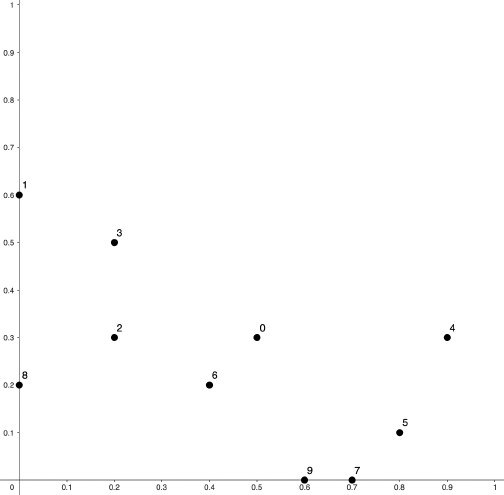
\includegraphics[width=0.35\linewidth]{images/skyline.png}
        \end{figure}
        We access the first row and since the window has no elements we add it to it. 
        We check for every tuple if it dominates the inserted one. 
        Only the tuples three and one are not dominated by the tuple four, so the final window contains the points four, three and one. 
        Graphically we have that the skyline of the given dataset is the following. 
        \begin{figure}[H]
            \centering
            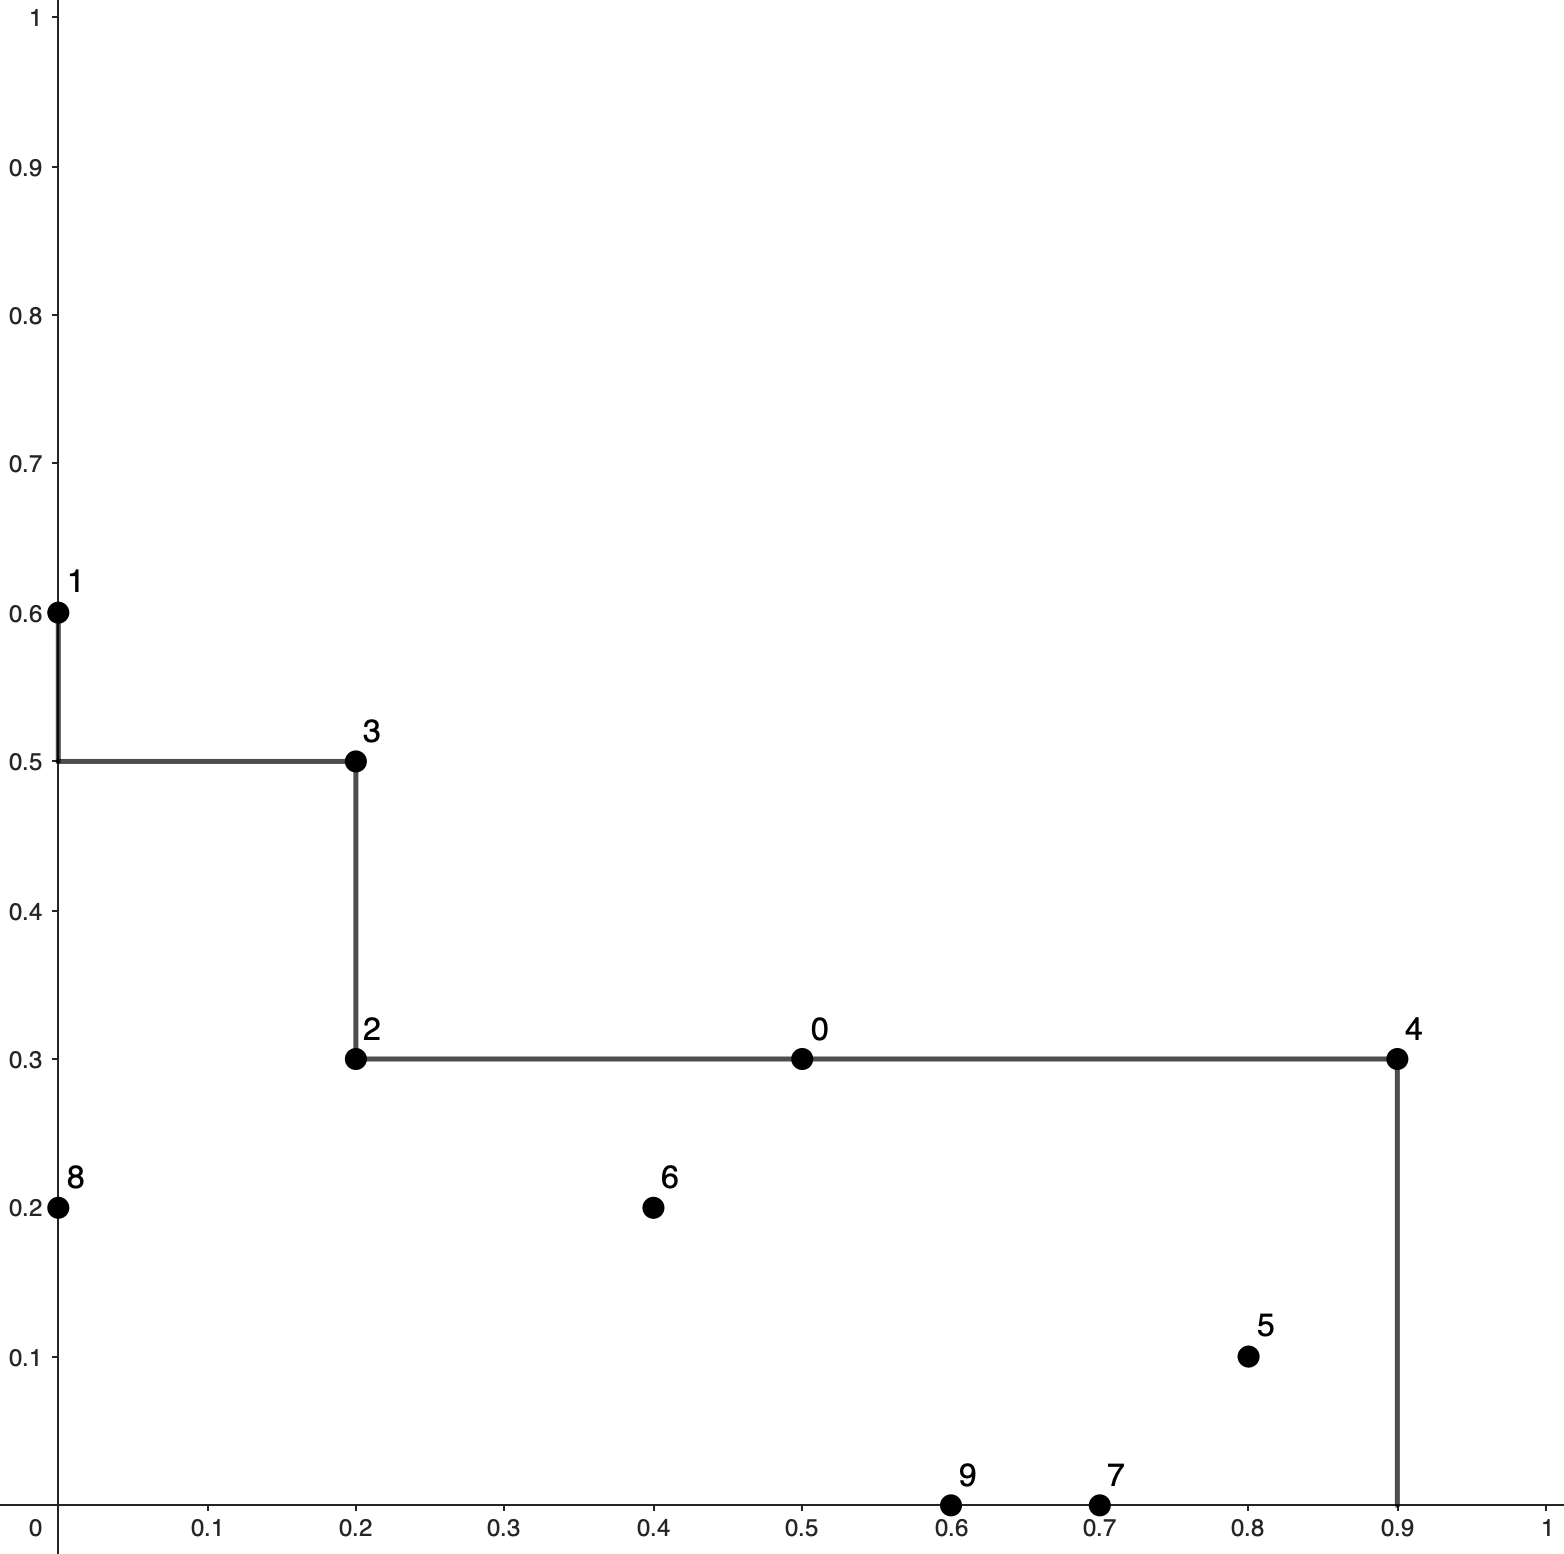
\includegraphics[width=0.35\linewidth]{images/skylinesol.png}
        \end{figure}
    \item Players zero and five are dominated only by player four, so they are part of the 2-skyband.
        Players one, three and four are part of the skyline, so they are obviously also part of the 2-skyband. 
        The 3-skyband is made of the players one, three, four, six and seven according to the definition. 
\end{enumerate}